\chapter{Mejora de las físicas en \textit{WebSim}}
\label{chap:motor_fisicas} 


En este capítulo se va a explicar el diseño, implementación y funcionamiento del nuevo motor de físicas complementario que se ha creado y que actualmente está en producción en el entorno \textit{Kibotics}. Como se detallará más adelante, el nuevo motor permite disponer de unas físicas más realistas en los ejercicios y simular nuevos escenarios, como rampas o pistas de hielo, ya que la gravedad y la fricción van a estar contempladas en la simulación. Además, se ganará utilidad a la hora de probar las soluciones de los ejercicos simulados en robots reales, puesto que los factores que presenta un robot físico (por ejemplo: masa, momento de incercia o velocidad máxima) o una escena real (por ejemplo: rozamiento estático, rozamiento dinámico, restitución o gravedad) van a ser parámetros que se puedan materializar en el simulador gracias a las novedades introducidas.


\section{Estudios previos: motor de físicas por defecto en \textit{A-Frame}}
\textit{A-Frame} utiliza por defecto el motor de  \textit{CANNON}\footnote{https://github.com/n5ro/aframe-physics-system} para materializar las físicas. \textit{CANNON} surgió como consecuencia de la necesidad de disponer de un motor de físicas en la web y presenta importantes semejanzas respecto a otros conocidos motores: \textit{three.js} o \textit{ammo.js}. Su ventaja es que su código se encuentra disponible enteramente en red\footnote{http://schteppe.github.io/cannon.js/docs/}, escrito en lenguaje \textit{JavaScript} y que su tamaño de archivo es considerablemente más pequeño que el de otros motores de físicas\footnote{http://schteppe.github.io/cannon.js/}.\newline

A continuación se detallan las posibilidades que ofrece \textit{A-Frame} para controlar la gravedad, la restitución y la fricción de una escena simulada.

\subsection{Gravedad} 
Dado que \textit{WebSim} se basa en la tecnología de \textit{A-Frame}, la gravedad es un parámetro configurable dentro de una escena. Los ficheros de configuración de los escenarios de los ejercicios en formato \textit{JSON} incluyen al principio del código las siguientes líneas que permiten seleccionar el valor deseado para la gravedad.

\begin{verbatim}
                    "scene": {
                        "gravity": -9.8
                    }
\end{verbatim}

Como se ha mencionado anteriormente, previamente al cambio introducido en las físicas, los ficheros de configuración de los ejercicios soportados en la plataforma tenían definida una gravedad con valor 0. Esta configuración era necesaria para conseguir hacer volar a los drones, puesto que con una gravedad de -9.8 cualquier cuerpo sólido de la escena caía hacia abajo como consecuencia de la atracción de la gravedad, por lo que no era posible hacer volar a los robots. Con el nuevo motor de físicas, todos los ejercicios están simulados con un valor de gravedad de -9.8.  \newline

\subsection{Colisiones}
Cualquier cuerpo sólido puede colisionar con otro cuerpo incluído en la escena simulada. Las colisiones pueden tener naturaleza elástica o inélastica dependiendo del valor del coeficiente de restitución de los objetos. El coeficiente de restitución es la media de la conservación de la energía cinética cuando se produce un choque entre partículas. Cuando su valor es 1 el choque es perfectamente elástico y cuando es 0, es perfectamente inelástico. 

\begin{equation}
   Coeficiente \,\, de \,\,restitución = \frac{Velocidad \,\, relativa \,\, tras \,\, la \,\, colisión}{Velocidad \,\, relativa \,\, antes \,\, de \,\, la \,\, colisión}
\end{equation} \newline

\textit{A-Frame} también ofrece la posibilidad de parametrizar el coeficiente de restitución. Este parámetro se puede configurar, al igual que la gravedad, al principio del fichero de configuración de los ejercicios incluyendo el siguiente código.

\begin{verbatim}
                    "scene": {
                        "physics": "restitution: 0.5"
                    }
\end{verbatim}

\subsubsection{Colisiones elásticas}
Se dice que una colisión es elástica cuando, tras el choque, se conserva toda la energía cinética. Esta se transfiere por completo desde el objeto que colisiona hasta el objeto que ha sido colisionado. En la realidad, en todo choque parte de la energía se disipa en calor, por lo que este tipo de colisiones es considerada ideal. Visualmente, el efecto que tiene es que el objeto que colisiona se queda parado y el objeto colisionado comienza a moverse a la velocidad que se movía el objeto que colisionó con él (si son de la misma masa). La Figura \ref{fig:elastico} muestra un ejemplo de colisión elástica.

\begin{figure}[h!]
    \centering
    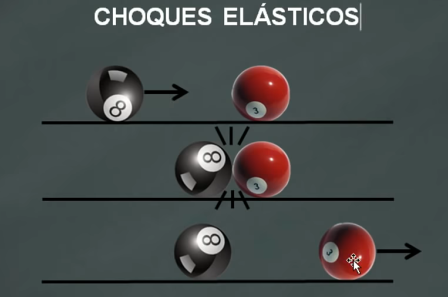
\includegraphics[width=0.7\textwidth, height=0.4\textwidth]{elastico.png}
    \caption[Colisión elástica]{Colisión elástica\footnotemark}
    \label{fig:elastico}
\end{figure}
\footnotetext{\url{https://www.youtube.com/watch?v=b9iOIr5DYj8}}


\subsubsection{Colisiones inelásticas}
Por otro lado, cuando se produce una colisión inelástica el objeto que colisiona continúa teniendo parte de la energía cinética, otra parte se transfiere al objeto que ha sido colisionado y la parte restante se disipa en forma de calor. En este tipo de choques el efecto visual es que tanto el objeto que colisiona como el objeto colisionado avanzan a cierta velocidad tras el choque. La Figura \ref{fig:inelastico} muestra un ejemplo de colisión inelástica.

\begin{figure}[h!]
    \centering
    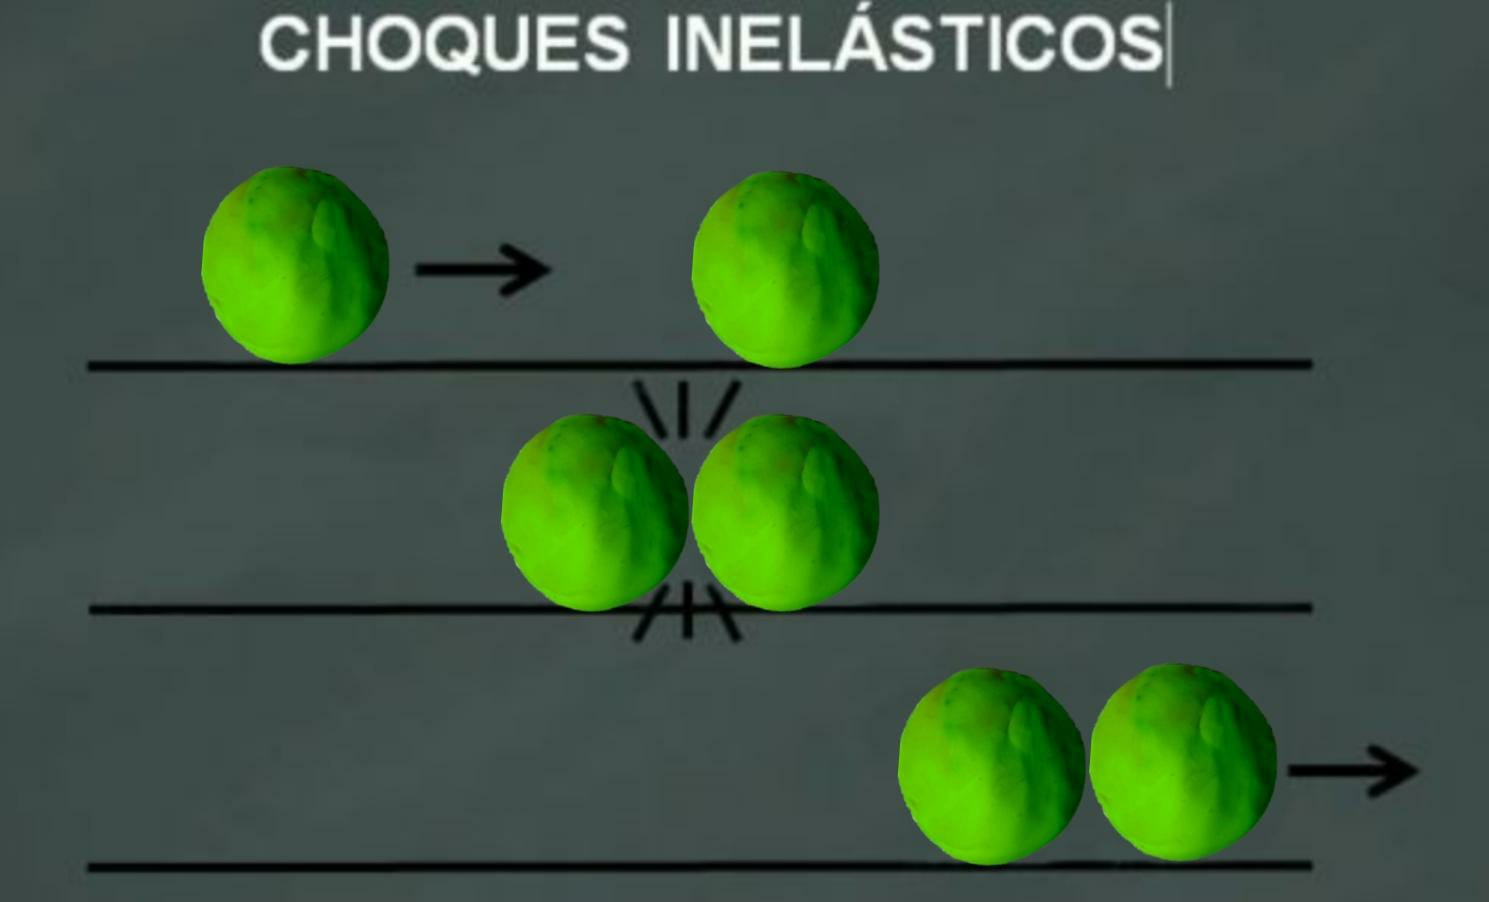
\includegraphics[width=0.7\textwidth, height=0.4\textwidth]{colision_inelastica.jpg}
    \caption[Colisión inelástica]{Colisión inelástica\footnotemark}
    \label{fig:inelastico}
\end{figure}
\footnotetext{Elaboración propia.}

\subsubsection{Pruebas de colisiones}
Se han realizado pruebas de colisiones de \textit{A-Frame} en tres escenarios diferentes variando el valor del coeficiente de restitución y la masa de los objetos. Los escenarios utilizados han sido los siguientes:

\begin{itemize}
    \item \textbf{Escenario 1:} dos pelotas cayendo por sendas rampas.
    \item \textbf{Escenario 2:} una pelota fija en el suelo y otra cayendo por una rampa.
    \item \textbf{Escenario 3:} una pelota cae por una rampa y colisiona con una pared.
\end{itemize}

\begin{figure}[!h]
  \begin{subfigure}[b]{0.3\textwidth}
    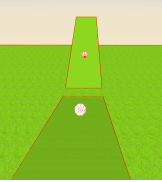
\includegraphics[width=\textwidth, height=\textwidth]{colision1.png}
    \caption{Escenario 1}
  \end{subfigure}
  \hfill
  \begin{subfigure}[b]{0.3\textwidth}
    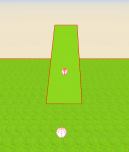
\includegraphics[width=\textwidth, height=\textwidth]{colision2.png}
    \caption{Escenario 2}
  \end{subfigure}
    \hfill
  \begin{subfigure}[b]{0.3\textwidth}
    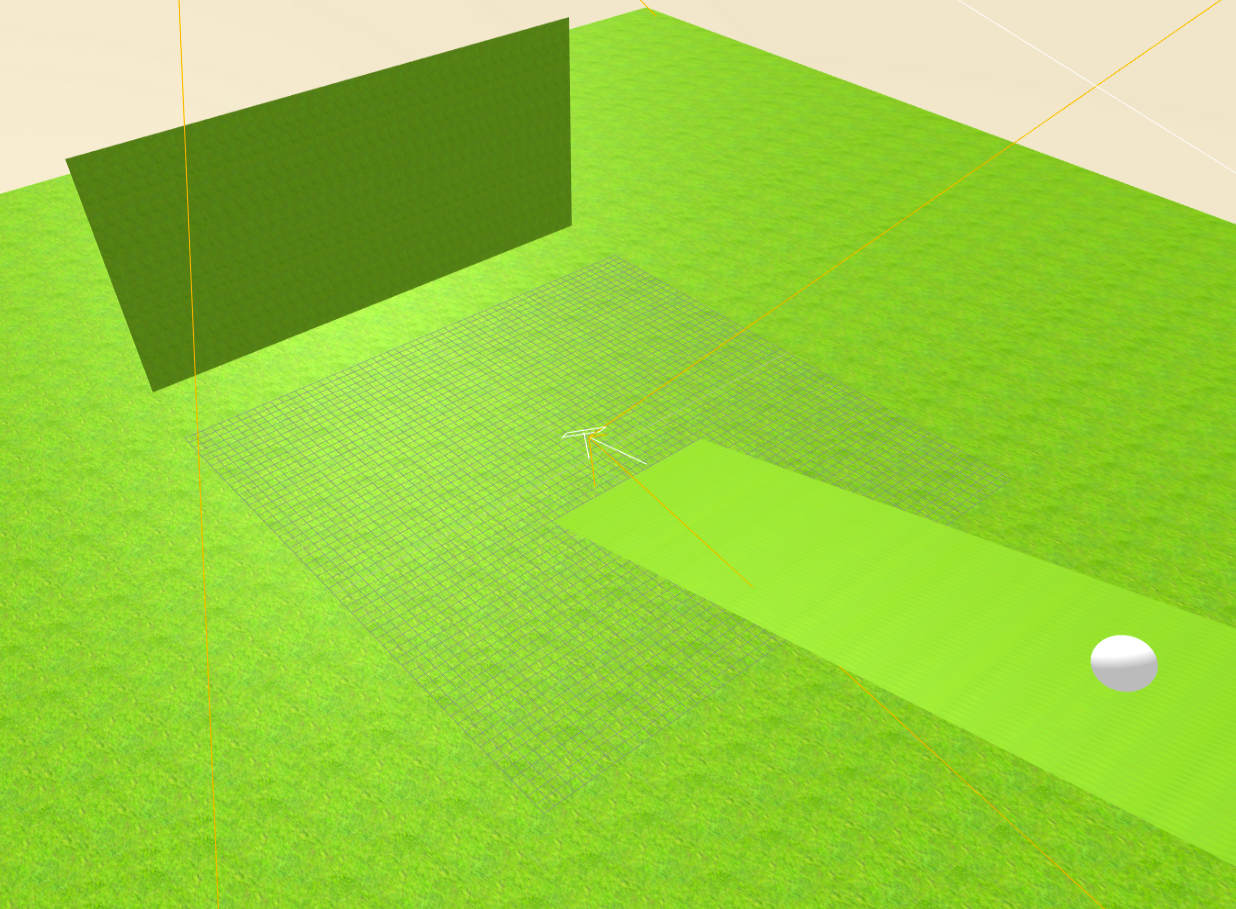
\includegraphics[width=\textwidth, height=\textwidth]{colision3.png}
    \caption{Escenario 3}
  \end{subfigure}
  \caption{Escenarios de prueba de las colisiones de \textit{A-Frame}}
 \end{figure}

Los resultados obtenidos durante las pruebas se detallan en los Cuadros \ref{fig:col-escenario1}, \ref{fig:col-escenario2} y \ref{fig:col-escenario3}. En este link\footnote{\url{https://youtu.be/T214FNFxehs}} se ofrece un vídeo con los resultados de las pruebas realizadas en el tercer escenario.
\begin{table}[]
\centering
 \resizebox{1.1\textwidth}{!}{  
\begin{tabular}{cc}
\hline
\multicolumn{1}{|c|}{\textbf{}}                 & \multicolumn{1}{c|}{\textbf{Misma masa}}                                                                                                                                    \\ \hline
\multicolumn{1}{|c|}{\textbf{Restitution = 0}}   & \multicolumn{1}{c|}{No hay rebote}                                                                                                                  \\ \hline
\multicolumn{1}{|c|}{\textbf{Restitution = 0.4}} & \multicolumn{1}{c|}{Sí hay rebote}                                                                         \\ \hline
\multicolumn{1}{|c|}{\textbf{Restitution = 1}}   & \multicolumn{1}{c|}{La pelota rebota al entrar en contacto con cualquier superfice de la escena}                                                                           \\ \hline
\multicolumn{1}{l}{}                            & \multicolumn{1}{l}{}                                                                                                                                                        \\ \hline
\multicolumn{1}{|l|}{}                          & \multicolumn{1}{c|}{\textbf{Diferente masa}}                                                                                                                                \\ \hline
\multicolumn{1}{|c|}{\textbf{Restitution = 0}}   & \multicolumn{1}{c|}{Las dos pelotas avanzan pegadas en la dirección de la de mayor masa}                                                                                    \\ \hline
\multicolumn{1}{|c|}{\textbf{Restitution = 0.4}} & \multicolumn{1}{c|}{La pelota más pesada hace cambiar la dirección del movimiento de la más ligera, que se desplaza a mayor velocidad} \\ \hline
\multicolumn{1}{|c|}{\textbf{Restitution = 1}}   & \multicolumn{1}{c|}{Las dos pelotas avanzan separadas en la dirección de la de mayor masa. La pelota de menor masa coge mayor velocidad}                                    \\ \hline
\end{tabular}
}
\caption{Resultados de las colisiones obtenidos con el escenario 1}
\label{fig:col-escenario1}
\end{table}

                                                                                                   
\begin{table}[]
\centering
 \resizebox{1.1\textwidth}{!}{  
\begin{tabular}{cc}
\hline
\multicolumn{1}{|c|}{\textbf{}}                 & \multicolumn{1}{c|}{\textbf{Misma masa}}                                                                                                                                                                                                                                                                                                                                                                               \\ \hline
\multicolumn{1}{|c|}{\textbf{Restitution = 0}}   & \multicolumn{1}{c|}{Ambas pelotas avanzan pegadas a la misma velocidad}                                                                                                                                                                                                                                                                              \\ \hline
\multicolumn{1}{|c|}{\textbf{Restitution = 0.4}} & \multicolumn{1}{c|}{La pelota que permanecía en el suelo se mueve más rápido que la que cayó por la rampa. No avanzan pegadas}                                                                                                                                                                                                                                                                           \\ \hline
\multicolumn{1}{|c|}{\textbf{Restitution = 1}}   & \multicolumn{1}{c|}{La pelota rebota al entrar en contacto con cualquier superfice de la escena}                                                                                                                                                                                                                                                                                                                      \\ \hline
\multicolumn{1}{l}{}                            & \multicolumn{1}{l}{}                                                                                                                                                                                                                                                                                                                                                                                                   \\ \hline
\multicolumn{1}{|l|}{}                          & \multicolumn{1}{c|}{\textbf{Diferente masa}}                                                                                                                                                                                                                                                                                                                                                                           \\ \hline
\multicolumn{1}{|c|}{\textbf{Restitution = 0}}   & \multicolumn{1}{l|}{\begin{tabular}[c]{@{}l@{}}- Masa pelota rampa $<$Masa pelota suelo: ambas pelotas se quedan juntas y paradas\\ - Masa pelota rampa $>$ Masa pelota suelo: ambas pelotas avanzan hacia adelante juntas y a la misma velocidad\end{tabular}}                                                        \\ \hline
\multicolumn{1}{|c|}{\textbf{Restitution = 0.4}} & \multicolumn{1}{l|}{\begin{tabular}[c]{@{}l@{}}- Masa pelota rampa $<$ Masa pelota suelo: la pelota que ha caído por la rampa rebota hacia arriba\\ - Masa pelota rampa $>$ Masa pelota suelo: la pelota que estaba en reposo avanza con más velocidad \\ que la que cayó por la rampa\end{tabular}} \\ \hline
\multicolumn{1}{|c|}{\textbf{Restitution = 1}}   & \multicolumn{1}{c|}{La pelota rebota al entrar en contacto con cualquier superfice de la escena}                                                                                                                                                                                                                                                                                                                      \\ \hline
\end{tabular}
}
\caption{Resultados de las colisiones obtenidos con el escenario 2}
\label{fig:col-escenario2}
\end{table}

\begin{table}[]
\centering
 \resizebox{1.1\textwidth}{!}{  
\begin{tabular}{cc}
\hline
\multicolumn{1}{|c|}{\textbf{}}                 & \multicolumn{1}{c|}{\textbf{Pelota con masa grande}}                                                                                       \\ \hline
\multicolumn{1}{|c|}{\textbf{Restitution = 0}}   & \multicolumn{1}{c|}{Permanece junto a la pared, sin rebote} \\ \hline
\multicolumn{1}{|c|}{\textbf{Restitution = 0.4}} & \multicolumn{1}{c|}{Sí hay rebote}                                                                       \\ \hline
\multicolumn{1}{|c|}{\textbf{Restitution = 1}}   & \multicolumn{1}{c|}{El rebote es muy elevado y vuelve a subir la rampa pŕacticamente a la misma velocidad que la bajó}         \\ \hline
                                                &                                                                                                                                \\ \hline
\multicolumn{1}{|c|}{}                          & \multicolumn{1}{c|}{\textbf{Pelota con masa pequeña}}                                                                                   \\ \hline
\multicolumn{1}{|c|}{\textbf{Restitution = 0}}   & \multicolumn{1}{c|}{Permanece junto a la pared, sin rebote}                                                                            \\ \hline
\multicolumn{1}{|c|}{\textbf{Restitution = 0.4}} & \multicolumn{1}{c|}{Cuanto más pequeña es la masa, más grande es el rebote}                                                                            \\ \hline
\multicolumn{1}{|c|}{\textbf{Restitution = 1}}   & \multicolumn{1}{c|}{Cuanto más pequeña es la masa, más grande es el rebote}                                                                            \\ \hline
\end{tabular}
}
\caption{Resultados de las colisiones obtenidos con el escenario 3}
\label{fig:col-escenario3}
\end{table}

 
\subsection{Fricción}
Cualquier cuerpo dinámico de una escena de \textit{A-Frame} presenta una fuerza de rozamiento que se opone al movimiento. Existen dos tipos de rozamiento: el rozamiento estático y el rozamiento dinámico. \textit{A-Frame} incluye tres parámetros diferentes que permiten variar el rozamiento de una superficie. No obstante, no se puede seleccionar un valor concreto para la fuerza de rozamiento estática y dinámica, ya que el atributo \textit{friction} hace variar los dos tipos de rozamiento en conjunto. Por tanto, se puede incrementar o disminuir tanto el rozamiento estático como el dinámico, pero no se pueden parametrizar con un valor concreto. \newline

Los ficheros de configuración de los escenarios de los ejercicios en formato \textit{JSON} incluyen al principio del código las siguientes líneas que permiten seleccionar el valor deseado para los atributos \textit{friction} (rozamiento estático y dinámico) y \textit{linear-damping y angular-damping} (rozamiento dinámico).

\small
\begin{verbatim}
                    "scene": {
                        "physics": "friction: 0.5"
                    }
                    attr": {
                        "static-body": {
                        "linearDamping":1.2,
                        "angularDamping":1.2
                    }
\end{verbatim}

\normalsize
\subsubsection{Rozamiento estático}
Dos superficies rígidas en reposo no se desplazan una respecto a la otra y cuando la fuerza paralela al plano tangente es suficientemente pequeña. Cuando el coeficiente de rozamiento estático de una superifice es excesivamente pequeño, los objetos que se encuentran sobre esa superficie sí se mueven con más facilidad. Una forma de calcular el coeficiente de rozamiento estático es hacer variar la inclinación de una rampa. Cuando se alcanza un ángulo de inclinación con el cual el cuerpo comienza a descender, se dice que se ha llegado al ańgulo critico. A partir del ángulo crítico se puede obtener el coeficiente de rozamiento estático gracias a la siguiente igualdad:

\begin{equation}
    tan(angulo \,\, crítico) = coeficiente \,\, de \,\, rozamiento \,\, estático \,\,
\end{equation}

\subsubsection{Rozamiento dinámico}
Cuando dos superficies están en contacto, el movimiento de una respecto a la otra genera fuerzas tangenciales llamadas fuerzas de fricción o rozamiento, las cuales tienen sentido opuesto al movimiento. La magnitud de esta fuerza depende del coeficiente de rozamiento dinámico. En \textit{A-Frame}, el rozamiento dinámico se puede configurar utilizando los atributos \textit{linear-damping y angular-damping} a nivel de objeto, además del atributo \textit{friction} a nivel de escena, como se ha mencionado anteriormente. 



\subsubsection{Pruebas de la fricción}
Se han realizado diferentes pruebas de fricción colocando un objeto en una rampa y variando la inclinación de la misma. Los resultados obtenidos han sido los siguientes:
\begin{itemize}
    \item \textbf{Prueba del rozamiento estático: } se coloca un objeto sobre una rampa y se procede a la variación de la inclinación de la misma. El objeto permanece en la misma posición hasta que se alcanza un ángulo de inclinación tan elevado que el cuerpo comienza a descender (ángulo crítico). Si se configura el atributo \textit{friction} con un valor más elevado, el ángulo crítico se alcanza más tarde, es decir, es mayor.
    \item \textbf{Prueba del rozamiento dinámico: } se mantiene fija la inclinación de la rampa y se varía el valor de los atributos \textit{friction, linear-damping y angular-damping}. Con unos valores elevados de esos tres parámetros, los robots no son capaces de subir la rampa. Sin embargo, a medida que se va reduciendo el valor de los atributos los robots comienzan a poder subir la rampa y cada vez lo hacen con mayor facilidad.
\end{itemize}

\section{Motor de físicas actual para robots en \textit{WebSim}}
Hasta el momento, \textit{WebSim} contaba con un motor de físicas completo. El movimiento de los robots se recreaba mediante la actualización de la posición cada 50 ms en función de la velocidad y la rotación consignada por el usuario. No entraban en juego aceleraciones ni fuerzas. Además, el hecho de actualizar la posición y la velocidad del robot constantemente (la velocidad se tomaba de manera instantánea de la última enviada por el cerebro software del robot. No existía diferencia entre la velocidad real y la velocidad deseada. Se asumía aceleración infinita del robot) sobreescribía encima de los cambios que introducía \textit{CANNON}, por lo que las físicas no incluían el efecto de la gravedad, la fricción ni el coeficiente de restitución. \newline 

La actualización de la posición de los robots en función de la velocidad y rotación comandadas se realizaba mediante la función \textit{updatePosition}.

\small{
\begin{verbatim} 

    updatePosition(rotation, velocity, robotPos) {
        if(simEnabled){
            let x = velocity.x / 10 * Math.cos(rotation.y * Math.PI / 180);
            let z = velocity.x / 10 * Math.sin(-rotation.y * Math.PI / 180);
            let y = (velocity.y / 10);
            robotPos.x += x;
            robotPos.z += z;
            robotPos.y += y;
        }
        return robotPos;
}
\end{verbatim}
}

\normalsize
La motivación de crear un motor de físicas complementario es que las físicas implementadas no recreaban un movimiento realista y no eran suficientes para lo que se tiene disponible en un robot real. Por ejemplo, los robots reales terrestres tienen que superar la fuerza de rozamiento para poder subir una rampa o los drones deben ser capaces de ejercer la fuerza necesaria para superar la gravedad y emprender el vuelo. Con un motor de físicas realistas, las soluciones implementadas en el simulador serán igualmente válidas para un robot físico y, además, permite la creación de ejercicios mucho más diversos, como una pista de hielo (en los que la fricción es extremadamente baja), arena (en los que la fricción es mucho más elevada) o escenarios multinivel con rampas (en los que los robots deberán ejercer fuerzas más grandes que en la superficie plana para poder ascender por la rampa). \newline

Las implicaciones que tiene la materialización de la gravedad y de la fricción son las siguientes:

\begin{itemize}
    \item \textbf{Materizalización de la gravedad:} los drones son capaces de volar en un mundo que materialice una gravedad de -9.8. Hasta el momento, los ejercicios de drones se configuraban con gravedad 0 para permitir volar al cuerpo.
    \item \textbf{Materialización de la fricción:} el desplazamiento de los robots no se realiza por imposición de una posición concreta, sino por la aplicación de la fuerza necesaria para alcanzar la velocidad objetivo. Al tener en cuenta la fricción, un robot deberá ejercer más fuerza sobre superficies con altas fricciones y menos fuerza en superficies con fricciones más pequeñas.
\end{itemize}

\clearpage
\section{Nuevo motor de físicas complementario}
\subsection{Diseño}
Este motor de físicas se utiliza para controlar el movimiento de los cuerpos dinámicos en la escena. Se le denomina complementario puesto que sólo se encarga de aplicar la fuerza autónoma al robot, dejando como tarea de \textit{CANNON} materializar las fuerzas de la fricción y la gravedad.

\begin{verbatim}
Fuerza robot = Fuerza autónoma + Fuerza gravedad + Fuerza fricción
\end{verbatim}

\begin{itemize}
    \item \underline{Fuerza gravedad:} materializada por \textit{CANNON} a un ritmo marcado por el propio motor \textit{CANNON}.
    \item \underline{Fuerza fricción:} materializada por \textit{CANNON} a un ritmo marcado por el propio motor \textit{CANNON}.
    \item \underline{Fuerza autónoma:} lo materializa nuestro motor complementario a su propio ritmo (distinto del de Cannon) y teniendo en cuenta las velocidades deseadas que marca en cada instante el código fuente del cerebro programado. El ritmo que se ha fijado ha sido de 20 ms.
\end{itemize}

Esta idea de motor complementario es radicalmente distinta de la implementación que existía hasta el momento. La función \textit{updatePosition} actúaba como un motor completo que sobreescribía a \textit{CANNON}. No existía combinación alguna entre ambos motores. \newline


La arquitectura del motor de físicas complementario presenta dos niveles. El nivel superior conecta directamente con el cerebro software del robot, el cual es capaz de dar continuamente instrucciones en posición y en velocidad. No obstante, ambos tipos de instrucciones se basan en comandar una velocidad objetivo. En el caso de las instrucciones en posición el robot se moverá a la velocidad objetivo hasta que se alcance la posición consignada en la instrucción y en el caso de las instrucciones en velocidad, el movimiento no termina. Este nivel más alto se basa en un controlador PD que traduce las consignas de velocidad que le llegan del cerebro, en la fuerza necesaria a aplicar al robot para alcanzar dichas velocidades consignadas. Estas fuerzas son las que entiende el núcleo o nivel más bajo del motor de físicas. Conociendo la masa y el momento de incercia, las fuerzas obtenidas se podrán traducir en aceleraciones. La Figura \ref{fig:motor_diseño} muestra un esquema del diseño del motor. \newline

Por otro lado, se incluye la tabla \ref{fig:parametros} que introduce a modo de resumen todos los parámetros que caraceterizan el movimiento
de los robots autónomos con el nuevo motor de físicas complementario. Tanto parámetros del modelo de fuerzas (masa, momento de inercia, fuerza máxima, torque máximo, maxima velocidad lineal, maxima velocidad angular, máxima aceleración lineal y máxima aceleración angular) como parámetros de \textit{A-Frame} (coeficiente de restitución, gravedad, fricción, amortiguación lineal y amortiguación angular). Los últimos ya se han explicado y los primeros se describen a continuación.

\begin{figure}[h!]
    \centering
    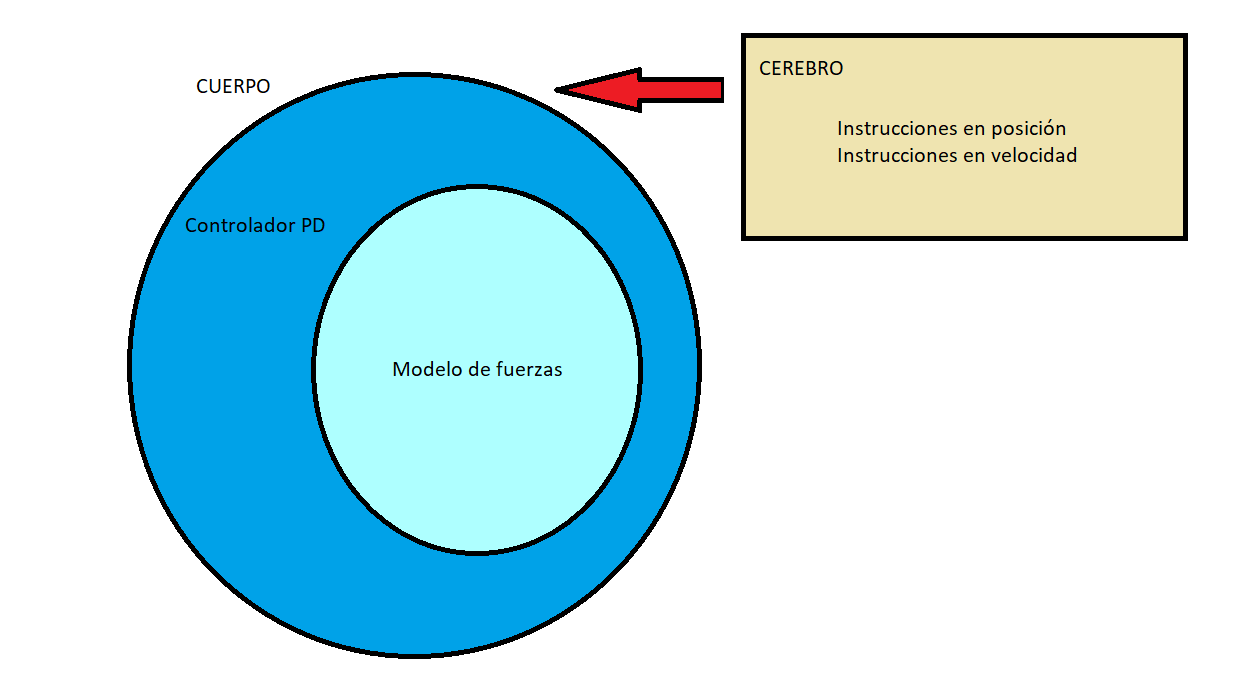
\includegraphics[scale=0.8]{Diseño_motor_4.PNG}
    \caption[Diseño del motor de físicas complementario]{Diseño del motor de físicas complementario\footnotemark}
    \label{fig:motor_diseño}
\end{figure}
\footnotetext{Elaboración propia.}

\begin{table}[h!]
\centering
\resizebox{15cm}{!}{
\begin{tabular}{|c|c|}
\hline
\multicolumn{2}{|c|}{\textbf{Parámetros del modelo de fuerzas}}                                                                          \\ \hline
mass                   & Masa del robot                                                                                                  \\ \hline
inertia                & Momento de inercia del robot                                                                                    \\ \hline
Fmax                   & Fuerza máxima aplicable                                                                                         \\ \hline
Tmax                   & Torque máximo aplicable                                                                                         \\ \hline
accelerationMax        & Aceleración lineal máxima                                                                                       \\ \hline
angularAccelerationMax & Aceleración angular máxima                                                                                      \\ \hline
linealSpeedMax         & \begin{tabular}[c]{@{}c@{}}Velocidad lineal máxima \\ que puede alcanzar el robot\end{tabular}                  \\ \hline
angularSpeedMax        & \begin{tabular}[c]{@{}c@{}}Velocidad angular máxima \\ que puede alcanzar el robot\end{tabular}                 \\ \hline
\multicolumn{2}{|c|}{\textbf{Parámetros de \textit{A-Frame}}}                                                           \\ \hline
restitution            & \begin{tabular}[c]{@{}c@{}}Conservación de la energía cinética \\ \\ en un choque entre partículas\end{tabular} \\ \hline
gravity                & Gravedad                                                                                                        \\ \hline
friction               & Fricción (rozamiento estático y dinámico)                                                                       \\ \hline
linearDamping          & \begin{tabular}[c]{@{}c@{}}Amortiguación lineal \\ (rozamiento dinámico en el movimiento lineal)\end{tabular}   \\ \hline
angularDamping         & \begin{tabular}[c]{@{}c@{}}Amortiguación angular \\ (rozamiento dinámico en el movimiento angular)\end{tabular} \\ \hline
\end{tabular}
}
\caption{Parámetros que caracterizan el movimiento de un robot autónomo}
\label{fig:parametros}
\end{table}

\clearpage
\subsection{Modelo de fuerzas}
El núcleo del nuevo motor de físicas es un modelo de fuerzas en el que, a partir de la definición de la masa y el momento de inercia del robot, se calcula la aceleración o torque a aplicar. De esta manera, un robot muy pesado deberá ejercer una fuerza mayor que un robot más ligero para alcanzar una misma velocidad. \newline

Para que el modelo funcione es necesaria la definición de los siguientes parámetros:
\begin{itemize}
    \item \textbf{Fuerza máxima:} es la fuerza autónoma máxima que puede aplicar un robot. Concede realismo al modelo, puesto que termina con la asunción de aceleración infinita.
    \item \textbf{Torque máximo:} es el momento autónomo de fuerza máximo que puede aplicar un robot, es decir, es la fuerza máxima de giro aplicable. Concede realismo al modelo, puesto que termina con la asunción de aceleración infinita.
    \item \textbf{Velocidad lineal máxima:} es la velocidad lineal máxima que puede alcanzar un robot.
    \item \textbf{Velocidad angular máxima:} es la velocidad angular máxima que puede alcanzar un robot.
    \item \textbf{Masa:} es necesaria para obtener el valor de la aceleración lineal.
    \item \textbf{Momento de inercia:} es la medida de la inercia rotacional cuando un cuerpo gira. Es el equivalente a la masa en un movimiento angular. Es necesario para obtener el valor de la aceleración angular.
\end{itemize}

\small
\begin{verbatim}

                /* Masa e incercia*/
                const mass = this.robot.body.mass;
                const inertia = this.robot.body.inertia.x;
                
                /* Fuerza y torque máximos */
                const fMax = 100;
                const tMax = 100;
                    
                    
                    
                /* Aceleración lineal y angular máxima */
                const accelerationMax = fMax / mass;
                const angularAccelerationMax = tMax / inertia;
                
                /* Aceleración lineal y angular máxima */
                const linearSpeedMax = 10;
                const angularSpeedMax= 5; 
                
                
\end{verbatim}



\subsection{Controlador PD}
\normalsize
El controlador PD se encarga de la traducción de las velocidades deseadas que le llegan al motor complementario en cada momento del cerebro a la fuerza autónoma a aplicar al robot. \newline

El controlador PD es una variante del controlador PID (controlador proporcional, integral y derivativo) que no incluye la componente integral. Se trata de un controlador por realimentación que calcula la desviación o error entre una medida y el valor que se desea obtener. Cada componente tiene una utilidad diferente y depende de distintos factores:
\begin{itemize}
    \item \textbf{Componente proporcional: }depende del error actual y su función es minimizar el error del sistema.
    \item \textbf{Componente derivativa: }depende de los errores pasados y permite estabilizar el sistema reduciendo la oscilación del valor de salida.
    \item \textbf{Componente integral: }es una predicción de los errores futuros y se utiliza cuando el componente derivativo no consigue reducir el error del sistema. Su uso es complejo ya que puede producir la desastibilización del sistema.
\end{itemize}

\clearpage
\begin{figure}[h!]
    \centering
    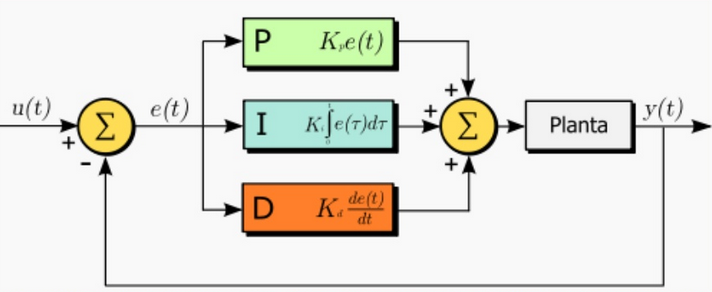
\includegraphics[scale=0.7]{pid.png}
    \caption[Controlador PID]{Controlador PID \footnotemark}
    \label{fig:pid}
\end{figure}
\footnotetext{https://es.slideshare.net/quasar.0360.7912/sintonizacion-de-controladores-pid}

Mediante un sencillo algoritmo basado en la suma de estos tres componentes, el controlador es capaz de ajustar su salida a un valor de referencia. Además, el modelo incluye tres constantes que se emplean para ponderar los componentes anteriores. En este caso sólo se van a tener en cuenta los componentes proporcionales y derivativos puesto que se van a implementar controladores PD  porque el error del sistema no es excesivamente elevado.\newline 

\begin{figure}[h!]
    \centering
    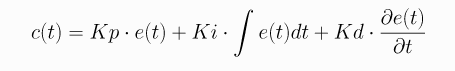
\includegraphics[scale=0.5]{pid_form.png}
    \label{fig:pid_form}
\end{figure}

Esta capa del motor incluye cuatro controladores PD diferentes que se ejecutan dependiendo del tipo de robot que esté realizando el movimiento (robot terrestre o drone) y del tipo de movimiento que se efectúe (avance lineal, giro, vuelo o suspensión en el aire). A continuación, se detallan los cuatro tipos de controladores incluidos.

\begin{itemize}
    \item \textbf{Controlador PD en velocidad del plano horizontal:} además de la velocidad horizontal deseada, coge como entrada la velocidad resultante del plano horizontal en ese instante y genera como salida la fuerza que debe ejercer el robot para alcanzar la velocidad objetivo. 
    
    \begin{figure}[h!]
    \centering
    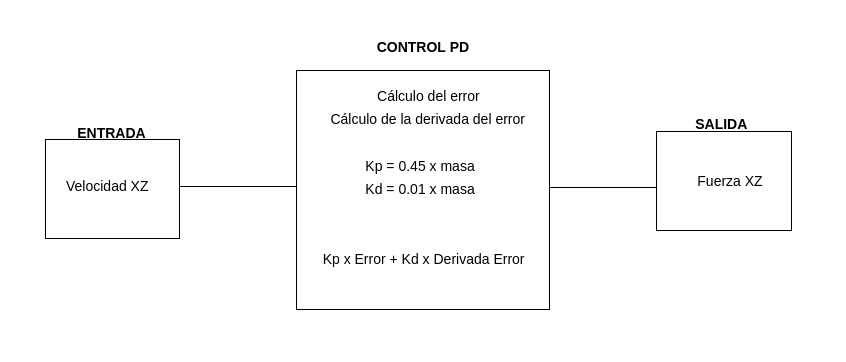
\includegraphics[width=\textwidth, height=0.4\textwidth]{controlador_PD_XZ.png}
    \caption[Diseño controlador PD en velocidad del plano horizontal]{Diseño controlador PD en velocidad del plano horizontal\footnotemark}
    \label{fig:esquema_pd_1}
    \end{figure}
    \footnotetext{Elaboración propia.}
    
    \item \textbf{Controlador PD en velocidad del eje vertical:} además de la velocidad vertical deseada, coge como entrada la componente vertical de la velocidad en ese instante y genera como salida la fuerza que debe ejercer el robot para alcanzar la velocidad objetivo. 
    
    \begin{figure}[h!]
    \centering
    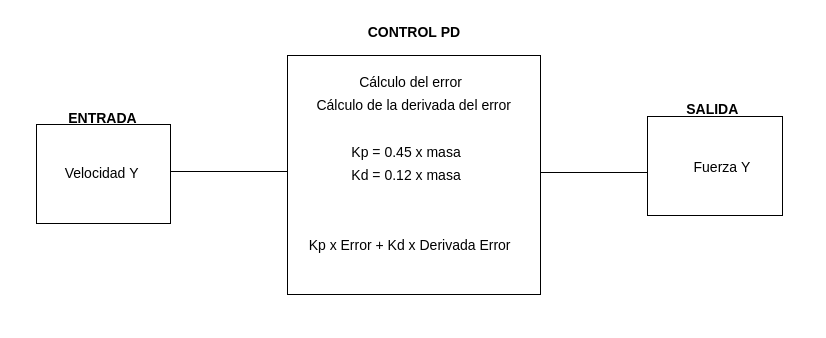
\includegraphics[width=\textwidth, height=0.4\textwidth]{controlador_PD_vel_Y.png}
\caption[Diseño controlador PD en velocidad del eje vertical]{Diseño controlador PD en velocidad del eje vertical\footnotemark}
    \label{fig:esquema_pd_2}
    \end{figure}
    \footnotetext{Elaboración propia.}
    
    \item \textbf{Controlador PD en velocidad angular horizontal (yaw):} además de la velocidad deseada de guiñada, coge como entrada la velocidad angular en ese instante y genera como salida el torque que debe ejercer el robot para alcanzar la velocidad de giro objetivo. 
    
    \clearpage
    \begin{figure}[h!]
    \centering
    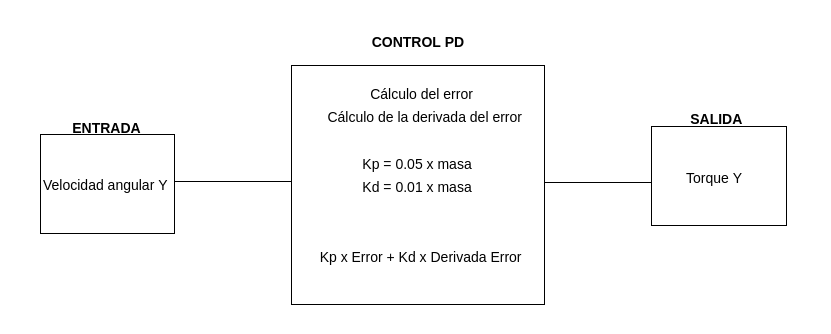
\includegraphics[width=\textwidth, height=0.4\textwidth]{control_PD_angular_drone.png}
\caption[Diseño controlador PD en velocidad angular horizontal para drone]{Diseño controlador PD en velocidad angular horizontal para drone\footnotemark}
    \label{fig:esquema_pd_3}
    \end{figure}
    \footnotetext{Elaboración propia.}

    \begin{figure}[h!]
    \centering
    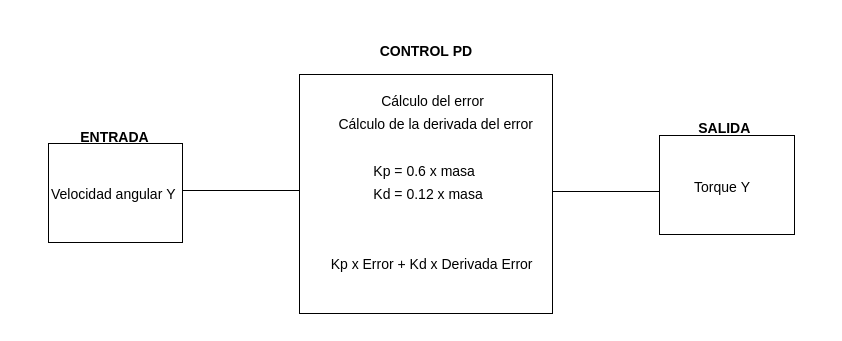
\includegraphics[width=\textwidth, height=0.4\textwidth]{control_PD_angular_tierra.png}
\caption[Diseño controlador PD en velocidad angular horizontal para robot terrestre]{Diseño controlador PD en velocidad angular horizontal para robot terrestre\footnotemark}
    \label{fig:esquema_pd_4}
    \end{figure} 
    \footnotetext{Elaboración propia.}
    
    \item \textbf{Controlador PD en posición para la altura:} coge como entrada la componente vertical de la posición en ese instante y genera como salida la fuerza que debe ejercer el robot para mantener una posición de referencia. Se usa cuando la velocidad deseada es cero. El control en velocidad vertical cuando la velocidad consignada es cero tiembla un poco, haciendo que el movimiento del drone pierda realismo. Por esta razón, se ha optado por materializar esa velocidad vertical cero con el control en posición vertical, con el que se obtiene un mejor resultado.
    
    \clearpage
    \begin{figure}[h!]
    \centering
    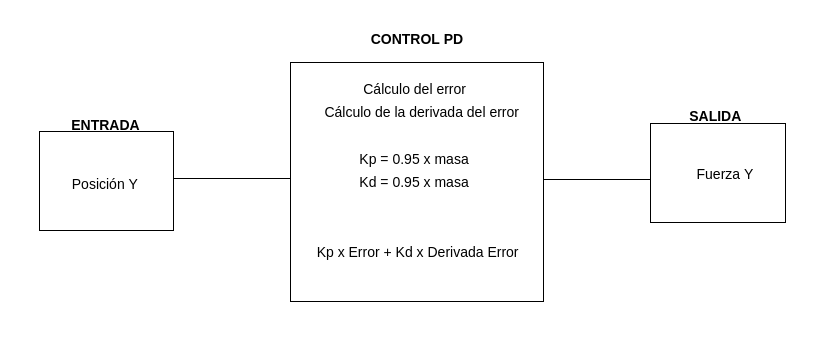
\includegraphics[width=\textwidth, height=0.4\textwidth]{controlador_PD_pos_Y.png}
    \caption[Diseño controlador PD en posición para la altura]{Diseño controlador PD en posición para la altura\footnotemark}
    \label{fig:esquema_pd_5}
    \end{figure}
    \footnotetext{Elaboración propia.}
\end{itemize}

De los controladores PD implementados, son específicos para el funcionamiento del drone el controlador PD en velocidad del eje vertical (empleado en el vuelo) y el controlador PD en posición para la altura (necesario cuando el robot debe permanecer inmóvil durante el vuelo en una posición concreta). El controlador PD en velocidad del plano horizontal es empleado en el movimiento lineal tanto de robots terrestres como de drones y el controlador PD en velocidad angular horizontal se utiliza durante los giros tanto de robots terrestres como de drones. No obstante, las constantes proporcional y derivativa y el torque máximo varían en función del tipo de robot, puesto que en el caso del drone la fricción no opone resistencia durante el giro, ya que este se encuentra volando sin mantener contacto con ninguna superficie.
    
\normalsize
\subsection{Timing}
Este concepto es de especial relevancia ya que es el que hace que el motor sea complementario y no completo, es decir, es lo que permite que el motor complementario se combine satisfactoriamente con el de \textit{CANNON} y no sobreescriba sus modificaciones. \newline

El motor de físicas complementario se ejecuta cada 20 ms gracias a un \textit{timeout} que lo invoca de forma periódica. Pero, ¿cuándo se ejecuta el motor de \textit{CANNON}? 

\small {
\begin{verbatim}
            setTimeout(this.auxiliaryPhysics.bind(this), 20);
\end{verbatim}
}

\normalsize
\textit{CANNON} actualiza sus físicas en cada iteración del bucle de renderizado de \textit{A-Frame}. Además, no lleva una cuenta explícita del tiempo y tampoco lo tiene en cuenta a la hora de modificar las posiciones y velocidades de los objetos de la escena. Puesto que la frecuencia de ejecución de \textit{CANNON} es superior a la del motor complementario, ha sido necesario calcular el número de veces que se ejecuta el código \textit{CANNON} entre dos iteraciones del motor de físicas complementario para poder realizar una correcta combinación entre ambos. El motor complementario deberá aplicar en cada iteración una aceleración X veces superior a la que corresponde, siendo X el número de veces que ha entrado \textit{CANNON} desde la útima vez que se ejecutó el motor complementario. \newline

\small {
\begin{verbatim}
    Aceleración autónoma = iteracionesCANNON x aceleración calculada
    
\end{verbatim}
}

\normalsize
El cómputo de las iteraciones de \textit{CANNON} se ha realizado creando un nuevo componente auxiliar que hace incrementar en uno un contador por cada tick de renderizado que ejecuta \textit{A-Frame}. \newline


Las variables y funciones que se han añadido al código original para llevar a cabo la implementación se incluyen a continuación. Las funciones \textit{tickCounter, getTickCounter y setTickCounter} se han utilizado para contabilizar el número de veces que se ejecuta el motor de \textit{CANNON} entre dos iteraciones del motor complementario.

\small {
\begin{verbatim}
                export var tickCounter = 0;
                
                export function getTickCounter() {
                    return tickCounter;
                }
                export function setTickCounter(value) {
                    tickCounter = value;
                }
\end{verbatim}
}

\normalsize
Para crear el nuevo componente auxiliar se han utilizado las herramientas que ofrece \textit{A-Frame} para el registro de nuevos componentes. La siguiente línea de código realiza el registro del nuevo componente auxiliar que se utiliza para contabilizar las iteraciones de \textit{CANNON}. A continuación, también se ha incluido el código del tick del nuevo componente registrado.

\small {
\begin{verbatim}


            /* Registro del nuevo componente */
            AFRAME.registerComponent("iterations", iterationsObj);
            
            /* Función tick del componente "iterations" */
            export var iterationsObj = {
                schema: {
                  count: { type: 'number', default: 0 },
                  position: { "x":0, "y":0, "z":0}
                },
                tick: function(){
                  setTickCounter(getTickCounter() + 1);
                  console.log('Tick de renderizado de A-FRAME');
                }
              }
            }
            
            
\end{verbatim}
}

\normalsize
Gracias a la correcta combinación temporal de ambos motores, se consigue que el motor de físicas complementario calcule la fuerza autónoma a aplicar a los robots dinámicos y \textit{CANNON} materialice la gravedad y fricción de la escena. La Figura \ref{fig:combi_motor} muestra la combinación existente actualmente entre ambos motores, que permite que se hable de un motor complementario y no de un motor completo. Cada motor lleva incorporado un reloj de ejecución independiente y, en el caso de \textit{CANNON}, es necesario disponer de un contador de ticks para monitorizar su hilo de ejecución.

\clearpage
\begin{figure}[h!]
    \centering
    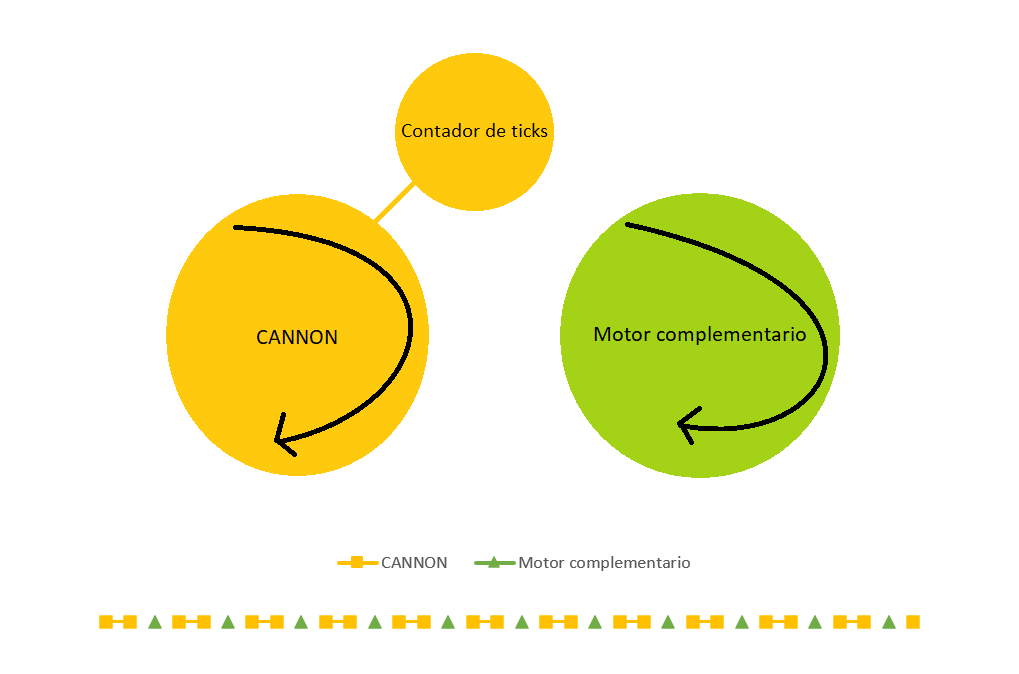
\includegraphics[scale=0.9]{combinacion_motores_2.PNG}
    \caption[Combinación de los motores de físicas a lo largo del tiempo]{Combinación de los motores de físicas a lo largo del tiempo\footnotemark}
    \label{fig:combi_motor}
\end{figure}
\footnotetext{Elaboración propia.}

\subsection{Implementación}
A continuación se incluyen los fragmentos de código que ha sido necesario incluir en el fichero \textit{interfacesRobot.js} del \textit{Simcore} de \textit{WebSim} para el correcto funcionamiento del motor complementario. \newline

\textbf{Adición de variables a la clase robot ya creada.} De esta manera, el motor complementario es escalable a ejercicios multirobot. Cada robot mantiene un registro propio del valor de sus variables.
\small {
\begin{verbatim}




                export class RobotI {
                    constructor(robotId) {
                        this.errorY = 0;
                        this.errorXZ = 0;
                        this.errorW = 0;
                        this.errorActualY = 0;
                        this.errorActualXZ = 0;
                        this.errorActualW = 0;
                        this.derivadaErrorY = 0;
                        this.derivadaErrorXZ = 0;
                        this.derivadaErrorW = 0;
                        this.forcePD = 0;
                        this.accelerationPD = 0;
                        this.commandedVelocityY = 0;
                        this.commandedVelocityXZ = 0;
                        this.commandedVelocityW = 0;
                        this.accelerationPDY = 0;
                        this.accelerationPDXZ = 0;
                        this.accelerationPDW = 0;
                        this.resultVelocity = 0;
                        this.refPos = 0;
                        this.init = true;
                        this.stop = true;
                        this.motorIterations = 0;
                }
                
                
                
                
                
                
                
                
\end{verbatim}
}

\normalsize
\textbf{Función auxiliaryPhysics.} Es la función que materializa el motor complementario y se ejecuta cada 20 ms gracias al \textit{timeout} que se ha añadido al final de la misma.

\footnotesize {
\begin{verbatim}
/*Actualización del contador de iteraciones*/
auxiliaryPhysics() {
    /* Control de velocidades máximas */
    var vmax = this.robot.getAttribute('vmax');
	var wmax = this.robot.getAttribute('wmax');
	if (this.robot.getAttribute('vmax') == null) {
	    var vmax = 10;
	}
	    
    if (this.robot.getAttribute('wmax') == null) {
        var wmax = 5;
	}
    this.motorIterations = getTickCounter(); 
               
    /* Sólo para Drone */
    /* Si la velocidad de vuelo objetivo es 0: */
    if ((this.velocity.y <= 0.0001) || (this.velocity.y <= -0.0001)){
        if (this.init == true) {
        /* Si el movimiento aún no ha comenzado la aceleración debe ser 0 */
            this.accelerationPDY = 0;
        } else { 
        /* Si el movimiento ya ha comenzado: */
    	    if (this.stop == true) {
    	/* Si se acaba de quedar en suspensión, guardo la posición de referencia */
    		  this.refPos = this.robot.body.position.y;
    		 }
    	/* Entra el controlador PD en posiciones */
            this.stop = false;
    		this.accelerationPDY = this.controladorPDVerticalPos();
    	}
    /* Si la velocidad objetivo no es 0, se ejecuta el controlador PD en velocidades */
    } else {
        this.init = false;
        this.stop = true;
        this.accelerationPDY = this.controladorPDVerticalVel();
    }
                
    /* Se utiliza la aceleración calculada con los controladores para obtener la 
    velocidad a aplicar utilizando las fórmulas MRUA y la combinación entre motores */
                
        this.commandedVelocityY = this.robot.body.velocity.y + 
        this.motorIterations*this.accelerationPDY;
        
	    if (Math.abs(this.commandedVelocityY) > vmax) {
            	if (this.commandedVelocityY > 0) {
                    this.commandedVelocityY = vmax;
            	} else {
                    this.commandedVelocityY = -vmax;
            	}
        }   
        
        this.robot.body.velocity.set(this.robot.body.velocity.x, 
        this.commandedVelocityY, this.robot.body.velocity.z); 
    }
    /* Movimiento en el plano horizontal: drone y robot terreste */
    
    /* Velocidad resultante = RaízCuadrada(Vx ² + Vz²)*/
	this.resultVelocity = Math.sqrt(Math.pow(this.robot.body.velocity.x, 2) + 
	Math.pow(this.robot.body.velocity.z, 2));
	
	/* Entra el controlador PD */
	this.accelerationPDXZ = this.controladorPDHorizontal(this.resultVelocity); 
	
	/* Se utiliza la aceleración calculada con los controladores para obtener la velocidad 
a aplicar utilizando las fórmulas MRUA y la combinación entre motores */
	this.commandedVelocityXZ = this.resultVelocity + 
	this.motorIterations*this.accelerationPDXZ;
	let rotation = this.getRotation();
	
	if (Math.abs(this.commandedVelocityXZ) > vmax) {
    	if (this.commandedVelocityXZ > 0) {
    	    this.commandedVelocityXZ = vmax;
    	} else {
    	    this.commandedVelocityXZ = -vmax;
        }
    }	
	
	/* La velocidad comandada resultante se descompone en las velocidades Vx y Vz */
	this.robot.body.velocity.set(this.commandedVelocityXZ*Math.cos(rotation.y*Math.PI/180), 
	this.robot.body.velocity.y,this.commandedVelocityXZ*Math.sin(-rotation.y*Math.PI/180));
	
    /* Movimiento angular: drone y robot terreste */
    
    /* Entra el controlador PD angular */              
    this.accelerationPDW = this.controladorPDAngular();
    
    /* Se utiliza la aceleración calculada con el controlador para obtener 
    la velocidad angular a aplicar utilizando las fórmulas MRUA y la 
    combinación entre motores */
    this.commandedVelocityW = this.robot.body.angularVelocity.y + 
    this.motorIterations*this.accelerationPDW;

    if (Math.abs(this.commandedVelocityW) > wmax) {
    	if (this.commandedVelocityW > 0) {
    	    this.commandedVelocityW = wmax;
        } else {
            this.commandedVelocityW = -wmax;
        }
    }     
    
    this.robot.body.angularVelocity.set(0, this.commandedVelocityW, 0);
    
    setTimeout(this.auxiliaryPhysics.bind(this), 20);
}





\end{verbatim}
}
\normalsize
\textbf{Controladores PD.} Se incluye como muestra del software implementado el controlador PD en velocidad del plano horizontal y el controlador PD en posición para la altura. Los controladores restantes presentan un código muy similar a estos.

\footnotesize {
\begin{verbatim}
/* Código del controlador PD en velocidad del plano horizontal */
    controladorPDHorizontal(resultVelocity) {
    /* Definición constantes para el controlador, fuerza máxima y aceleración máxima */
        const kp = 0.45;
        const kd = 0.01;
        const mass = this.robot.body.mass;
        var fMax = this.robot.getAttribute('fmax');
        if (this.robot.getAttribute('fmax') == null) {
	    	var fMax = 1000000;
	    }
        const accelerationMax = fMax / mass;

        /* Cálculo del error y derivada del error*/
        this.errorActualXZ = this.velocity.x - resultVelocity;
        this.derivadaErrorXZ = this.errorActualXZ - this.errorXZ;
        this.errorXZ = this.errorActualXZ;

        /* Salida del controlador */
        this.forcePD = kp*this.errorActualXZ + kd*this.derivadaErrorXZ;
        
        /* Obtención de la aceleración teniendo en cuenta la masa */
        this.accelerationPD = this.forcePD / mass;

        /* Límite de aceleración aplicable en cada iteración */
        if (Math.abs(this.accelerationPD) > angularAccelerationMax) {
            if (this.accelerationPD > 0) {
                this.accelerationPD = angularAccelerationMax;
            } else {
                this.accelerationPD = - angularAccelerationMax;
            }
        }
        return this.accelerationPD;
    }
\end{verbatim}
}

\footnotesize {
\begin{verbatim}  
/* Código del controlador PD en posición para la altura*/
    controladorPDVerticalPos() {
        /* Definición constantes para el controlador, fuerza máxima y                   aceleración máxima */
        const kp = 0.95;
        const kd = 0.95;
        const mass = this.robot.body.mass;
        var fMax = this.robot.getAttribute('fmax');
        if (this.robot.getAttribute('fmax') == null) {
	    	var fMax = 1000000;
	    }
        const accelerationMax = fMax / mass;
        

        /* Cálculo del error y derivada del error*/
        this.errorActualY = this.refPos - this.robot.body.position.y;
        this.derivadaErrorY = this.errorActualY - this.errorY;
        this.errorY = this.errorActualY;
        
        /* Salida del controlador */
        this.forcePD = kp*this.errorActualY + kd*this.derivadaErrorY;
        
        /* Obtención de la aceleración teniendo en cuenta la masa */
        this.accelerationPD = this.forcePD / mass;

        /* Límite de aceleración aplicable en cada iteración */
        if (Math.abs(this.accelerationPD) > angularAccelerationMax) {
            if (this.accelerationPD > 0) {
                this.accelerationPD = angularAccelerationMax;
            } else {
                this.accelerationPD = - angularAccelerationMax;
            }
        }
        return this.accelerationPD;
    }
}
\end{verbatim}
}

\normalsize
\section{Validación experimental}
\subsection{Simulación realista de robots terrestres}
El motor de físicas complementario permite dotar a \textit{WebSim} de un motor de físicas más realistas puesto que únicamente actúa sobre la fuerza autónoma del robot, dejando libertad a \textit{CANNON} para materializar tanto fricción como gravedad. Gracias a ello, se simulan mundos en los que los requisitos se asemejan en mayor medida a las características que se encuentran en el mundo real y en los robots físicos. \newline

En consecuencia, se van a poder desarrollar ejercicios más variados como pistas de hielo o ejercicios multinivel con rampas que interconecten los múltiples niveles. El modelo de físicas es ahora mucho más realista, pero hay que configurarlo adecuadamente para
cada robot eligiendo valores apropiados para sus parámetros. A continuación, se incluyen varios ejemplos en los que se puede observar cómo, con una correcta configuración de los atributos, se puede lograr la simulación de situaciones muchos más diversas y realistas:

\begin{itemize}

  \item \textbf{Fuerza máxima = 0.1.} No es posible ascender por una rampa dado que la fuerza máxima del mBot no es suficiente para superar la fricción. Esta situación puede solucionarse disminuyendo la fricción de la escena, reduciendo la inclinación de la rampa o aumentando la fuerza máxima del robot\footnote{\url{https://youtu.be/LQk9GLoMIk0}}.
    
    \begin{figure}[h!]
  \begin{subfigure}[b]{0.3\textwidth}
    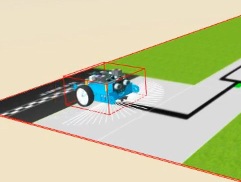
\includegraphics[width=\textwidth, height=\textwidth]{rampa1.png}
  \end{subfigure}
  \hfill
  \begin{subfigure}[b]{0.3\textwidth}
    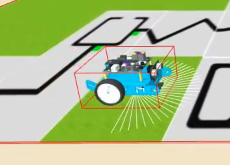
\includegraphics[width=\textwidth, height=\textwidth]{rampa 2.png}
  \end{subfigure}
    \hfill
  \begin{subfigure}[b]{0.3\textwidth}
    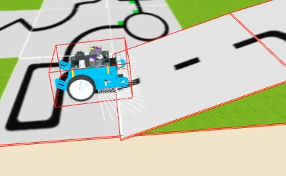
\includegraphics[width=\textwidth, height=\textwidth]{rampa3.png}
  \end{subfigure}
\caption{Subida de rampa con una fuerza máxima insuficiente}
\label{fig:rampa}
\end{figure}
    \item \textbf{Fricción = 0.00000001.} El escenario se puede asimilar a una pista de hielo. Cuando se le consigna al robot una instrucción en posición, por ejemplo 'gira 90º a la izquierda', se observa cómo el robot no es capaz de frenar el movimiento a los 90º a pesar de que su controlador PD angular comienza a comandar fuerzas para tratar de frenarlo. Sin embargo, como la fricción es excesivamente pequeña el controlador tarda más tiempo en lograr frenar el movimiento, tal y como ocurriría en una pista de hielo\footnote{\url{https://www.youtube.com/watch?v=QfPmtPeEL5k}}. La Figura \ref{fig:pistahielo} muestra la ejecución de esta instrucción y se observa cómo el robot finaliza el movimiento prácticamente a los 180º por esta razón.

\begin{figure}[h!]
  \begin{subfigure}[b]{0.5\textwidth}
    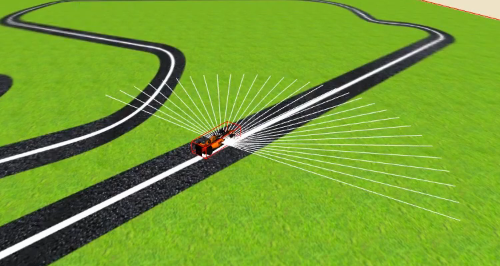
\includegraphics[width=\textwidth, height=\textwidth]{pistahielo1.png}
  \end{subfigure}
  \hfill
  \hfill
  \begin{subfigure}[b]{0.5\textwidth}
    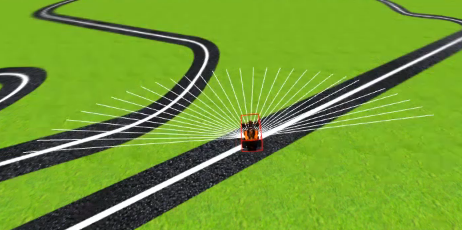
\includegraphics[width=\textwidth, height=\textwidth]{pistahielo2.png}
  \end{subfigure}
    \hfill
    \hfill
  \begin{subfigure}[b]{0.5\textwidth}
    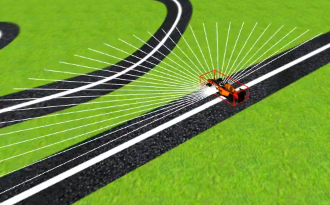
\includegraphics[width=\textwidth, height=\textwidth]{pistahielo3.png}
  \end{subfigure}
    \hfill
  \begin{subfigure}[b]{0.5\textwidth}
    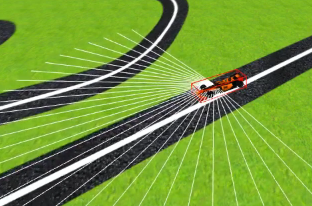
\includegraphics[width=\textwidth, height=\textwidth]{pistahielo4.png}
  \end{subfigure}
\caption{Giro de 90º hacia la izquierda en una superficie con una fricción muy baja}
\label{fig:pistahielo}
\end{figure}
\end{itemize}

La Figura \ref{fig:friccion-acele} muestra cómo influye en la aceleración autónoma que aplica el motor de físicas complementario el valor de fricción que se parametrice en el escenario. Cuanto mayor es la fricción, más grande es la aceleración autónoma que se debe aplicar.

\begin{figure}[h!]
    \centering
    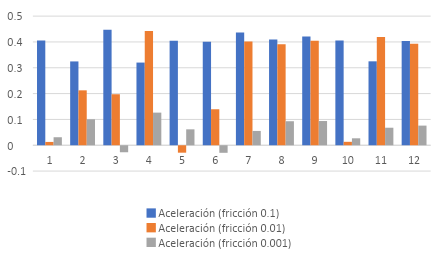
\includegraphics[scale=0.8]{aceleracion-friccion.png}
    \caption{Relación fricción - aceleración}
    \label{fig:friccion-acele}
\end{figure}

Por último, la Figura \ref{fig:vel-planoXZ} muestra la diferencia entre la progresión de la velocidad a lo largo del tiempo con y sin el motor de físicas complementario. Se observa que con el motor de físicas complementario la velocidad tarda unos milisegundos en estabilizarse y que cada vez se va ajustando mejor al valor objetivo. Sin embargo, la curva que genera la simulación sin el motor complementario es absolutamente irreal, ya que se está asuminedo una aceleración infinita.

\begin{figure}[h!]
    \centering
    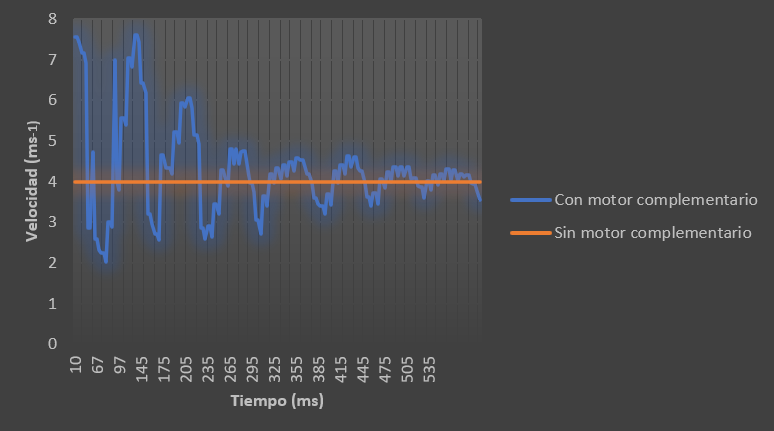
\includegraphics[scale=0.8]{PD_vel_XZ.PNG}
    \caption{Tiempo - Velocidad Controlador PD en velocidad del plano horizontal}
    \label{fig:vel-planoXZ}
\end{figure}

\newpage
\subsection{Simulación realista de drones}
El motor de físicas complementario dota a \textit{WebSim} de unas físicas más realistas puesto que permite a \textit{CANNON} materializar la gravedad. Gracias a ello, se pueden simular mundos en los que, a pesar de existir una gravedad de -9.8, la fuerza autónoma que hace aplicar el motor complementario permite volar al drone. \newline

Las físicas realistas implementadas permiten diferenciar entre el despegue de un drone ligero y el de uno mucho más pesado. Por ejemplo, para un fuerza máxima de 1 N, un drone de 1 Kg podrá despegar mientras que otro de 100 Kg no será capaz puesto que la fuerza máxima aplicada no es suficiente para superar la fuerza de la gravedad\footnote{\url{https://www.youtube.com/watch?v=S1E1zKjFkLo}}.

\begin{figure}[h!]
  \centering
  \begin{subfigure}[b]{\textwidth}
    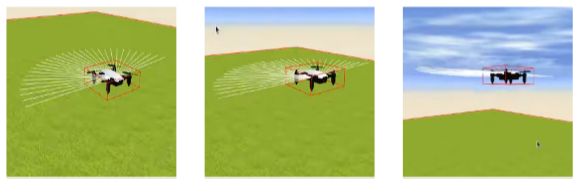
\includegraphics[scale=0.8]{masadrone_1.png}
    \caption{Despegue del drone Tello de 1 Kg}
  \end{subfigure}
  \hfill
  \begin{subfigure}[b]{\textwidth}
    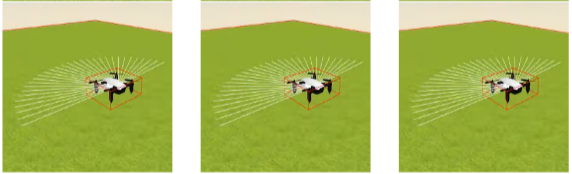
\includegraphics[scale=0.8]{dronemasa_2.png}
    \caption{Despegue del drone Tello de 100 Kg}
  \end{subfigure}
\caption{Despegue con drones de diferentes masas}
\label{fig:masadrone}
\end{figure}


Por otro lado, el control PD en posición incrementa el realismo de las físicas también a nivel visual puesto que hace recrear un movimiento más fluido y no produce una brusca frenada como ocurría con la imposición de la posición con \textit{updatePosition}. La fluidez del movimiento se consigue gracias a la fase de estabilización característica del controlador PD hasta que consigue aproximar su salida al valor de referencia\footnote{\url{https://www.youtube.com/watch?v=jSGI6KJbzTQ}}. En la Figura \ref{fig:pos-ejeY} se aprecia cómo el controlador tarda unos ms en estabilizar la posición y al principio la posición tiende a caer como consecuencia de la atracción de la gravedad. La Figura \ref{fig:vel-ejeY} muestra la progresión de la velocidad a lo largo del tiempo cuando el drone despega.

\begin{figure}[h!]
    \centering
    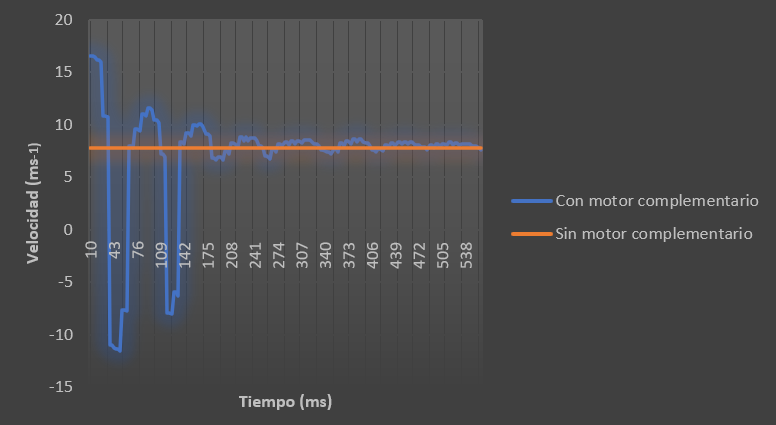
\includegraphics[scale=0.8]{PD_pos_Y.PNG}
    \caption{Tiempo - Posición Controlador PD en posición para la altura}
    \label{fig:pos-ejeY}
\end{figure}

\begin{figure}[h!]
    \centering
    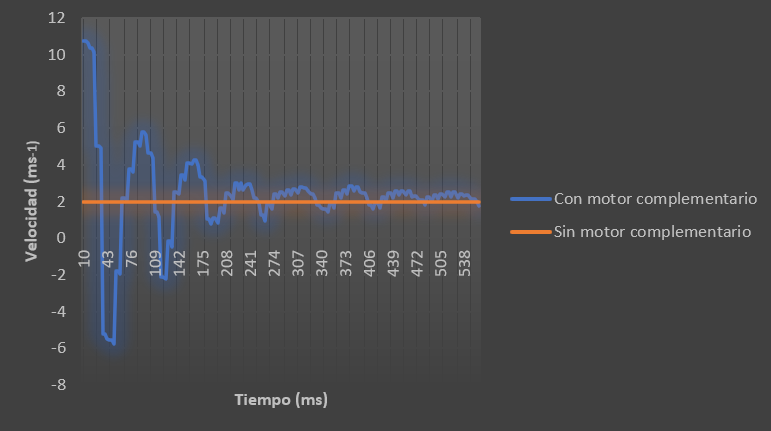
\includegraphics[scale=0.8]{PD_vel_Y.PNG}
    \caption{Tiempo - Velocidad Controlador PD en velocidad del eje vertical}
    \label{fig:vel-ejeY}
\end{figure}

